\AtBeginSection{}
%%%%%%%%%%%%%%%%%%%%%%%%%%%%%%%%%%%%%%%%%%%%%%%%%%%%%%%%%%%%%%%%%%%%%%%%
\section{Dokumentation}
\begin{frame}
  \frametitle{\kap. Dokumentation}%
\tableofcontents[current]
\end{frame}
% \setcounter{section}{0}


%%%%%%%%%%%%%%%%%%%%%%%%%%%%%%%%%%%%%%%%%%%%%%%%%%%%%%%%%%%%%%%%%%%%%%%%
\def\stitle{Java SE 8 Dokumentation}%
\subsection*{\stitle}\label{S:Java SE 8 Dokumentation}
\begin{frame}[t]%
  \frametitle{\kap.\ref{S:Java SE 8 Dokumentation} \stitle}%
\medskip

\begin{itemize}
\item Vollst\"andige Dokumentation \textcolor{KITblue}{\url{http://docs.oracle.com/javase/8/docs/api/}}
\item Umfassende Internet Tutorien \textcolor{KITblue}{\url{https://www.tutorialspoint.com/java/}} oder \textcolor{KITblue}{\url{https://www.javatpoint.com/java-tutorial}}
\end{itemize}
\medskip

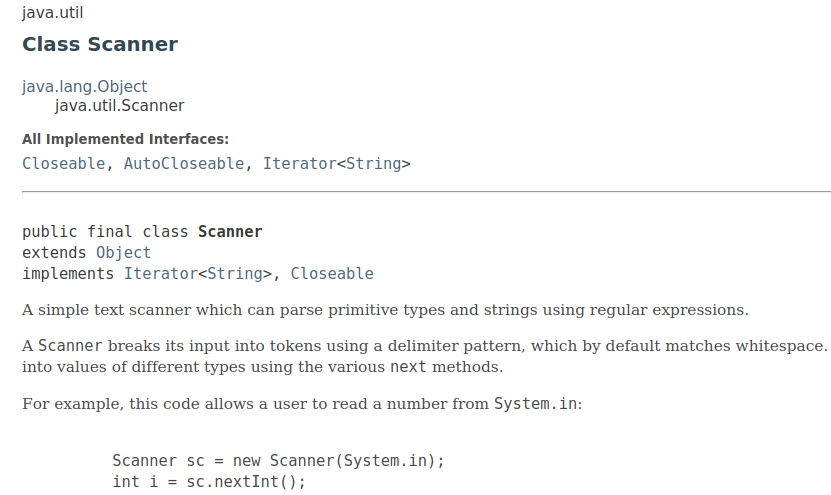
\includegraphics[width=0.8\textwidth]{javaDokumentation/java_small.png}
\end{frame}


%%%%%%%%%%%%%%%%%%%%%%%%%%%%%%%%%%%%%%%%%%%%%%%%%%%%%%%%%%%%%%%%%%%%%%%%
\def\stitle{Online Compiler}%
\subsection*{\stitle}\label{S:Online Compiler}
\begin{frame}[t]%
  \frametitle{\kap.\ref{S:Online Compiler} \stitle}%
\medskip

Auf der Seite \textcolor{KITblue}{\url{https://www.compilejava.net}} k\"onnen Sie sehr bequem kleinere Programme compilieren und ausf\"uhren.
Einzige Voraussetzung ist dabei eine bestehende Internet Verbindung.
\end{frame}
